\section{Resultados}
\label{sec:resultados}

Las secciones siguen el orden de la Sección~\ref{sec:organizacion}.
Salvo indicación en contrario, los experimentos usan los parámetros de la
Sección~\ref{sec:parametros}, y todos los números son trazables a corridas del sistema
actual (Sección~\ref{sec:auditoria}).

% ---------------------------------------------------------------
\subsection{Calibración del directorio a ocho módulos}
\label{sec:calibracion}

La calibración mide cómo debe leerse el directorio para que el enrutamiento maduro sea
confiable.
Se compararon nueve condiciones: la lectura cruda (A), dos normalizaciones por el conteo
de registros de cada módulo (B1, B2) y seis que actúan sobre otra cosa: un tope de
registros por módulo (C), consultas balanceadas (D), la cuantización (E32, E64), el
vocabulario (F) y la combinación de D, B1 y F (G).
Cada una se evaluó sobre el banco de 411 consultas, con $N \in \{50, 100, 200, 400\}$
consultas para formar el directorio y 5 semillas por celda.
La Tabla~\ref{tab:calibracion} da los resultados en $N = 400$; la
Figura~\ref{fig:mature-vs-n} muestra cómo crece la precisión madura con $N$, y la
Figura~\ref{fig:heatmap-condicion} da los mismos valores como mapa de calor.

En este estudio, como en el protocolo completo y en la curva de formación, la fase
madura se evalúa sobre las mismas $N$ consultas cuyos tokens formaron el directorio:
mide si el directorio reproduce lo que registró, no si generaliza a consultas nuevas.
Sobre 171 consultas reservadas, el protocolo transactivo del experimento 11 enruta
correctamente el 97.0\% con 200 imágenes por clase (Sección~\ref{sec:eham-unica}).

\begin{table}[H]
    \centering
    \caption{Precisión bajo distintas condiciones de lectura del directorio
    ($N = 400$, media de 5 semillas, 400 consultas del banco de 411).
    La precisión temprana no depende de la lectura del directorio, por lo que solo
    varía en las condiciones que alteran las consultas (D, G).
    F coincide con A: el vocabulario por masa asociativa no contiene las etiquetas
    polisémicas (las de Apple~Inc.) que la depuración quitaría.}
    \label{tab:calibracion}
    \small
    \setlength{\tabcolsep}{4pt}
    \begin{tabular}{llccc}
        \toprule
        Condición & Descripción & Temprana (\%) & Fidelidad (\%) & Madura (\%) \\
        \midrule
        A (cruda)  & Puntuación de activación sin normalizar        & 90.0 & 90.5 & 85.2 \\
        B1         & División entre conteo de registros por módulo  & 90.0 & 95.8 & \textbf{93.0} \\
        B2         & División entre raíz cuadrada del conteo        & 90.0 & 95.2 & 91.8 \\
        C          & Tope de registros por módulo                   & 90.0 & 91.2 & 88.0 \\
        D          & Consultas balanceadas entre clases             & 90.5 & 91.4 & 87.3 \\
        E32        & Cuantización en 32 niveles                     & 90.0 & 92.2 & 88.5 \\
        E64        & Cuantización en 64 niveles                     & 90.0 & 93.0 & 89.8 \\
        F          & Vocabulario depurado ($\equiv$ A)              & 90.0 & 90.5 & 85.2 \\
        G          & D + B1 + F                                     & 90.5 & 95.7 & 93.5 \\
        \bottomrule
    \end{tabular}
\end{table}

\paragraph{B1 es la corrección que no se puede sustituir.}
La lectura cruda del directorio (A) pierde 7.8 puntos frente a la lectura B1 (85.2\%
frente a 93.0\%).
Ninguna de las condiciones que actúan sobre los síntomas del sesgo y no sobre su causa
(B2, C, D, E32, E64) alcanza a B1; la más cercana, B2, queda a 1.2 puntos.
La combinación G supera a B1 por medio punto (93.5\% frente a 93.0\%), menos de lo que
G varía entre semillas (de 93.0 a 93.7\%; B1 da lo mismo con todas): una vez que la
puntuación mide evidencia por registro y no evidencia total, balancear las consultas y
depurar el vocabulario aportan poco.

\begin{figure}[H]
    \centering
    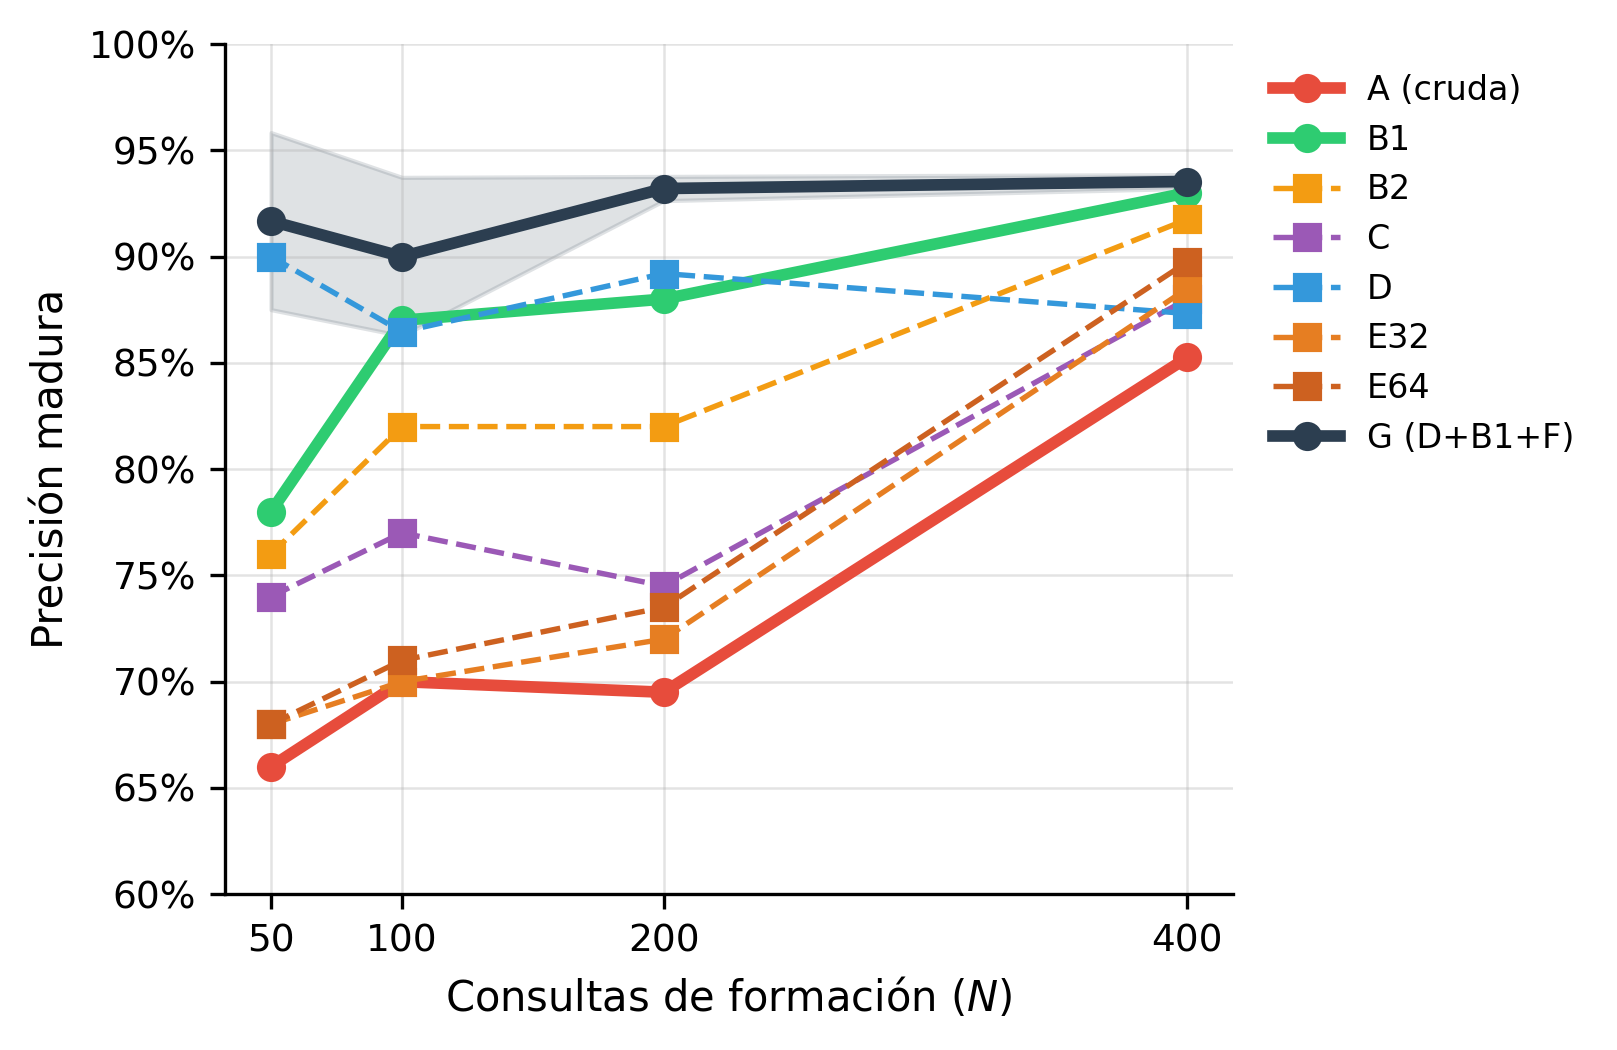
\includegraphics[width=0.9\textwidth]{fig02_mature_accuracy_vs_N.png}
    \caption{Precisión madura en función de $N$ para las condiciones de la
    Tabla~\ref{tab:calibracion} ($N$ consultas del banco de 411, media de 5 semillas; la
    banda es $\pm 1$ desviación estándar de G).
    Entre las condiciones que solo cambian la lectura, B1 es la mejor en todo el rango y
    la cruda (A) queda por debajo.
    G, que además balancea las consultas, queda por encima de B1 en todo el rango; D lo
    supera en $N = 50$ y $200$.
    F coincide con A en todos los puntos y no se dibuja.}
    \label{fig:mature-vs-n}
\end{figure}

\begin{figure}[H]
    \centering
    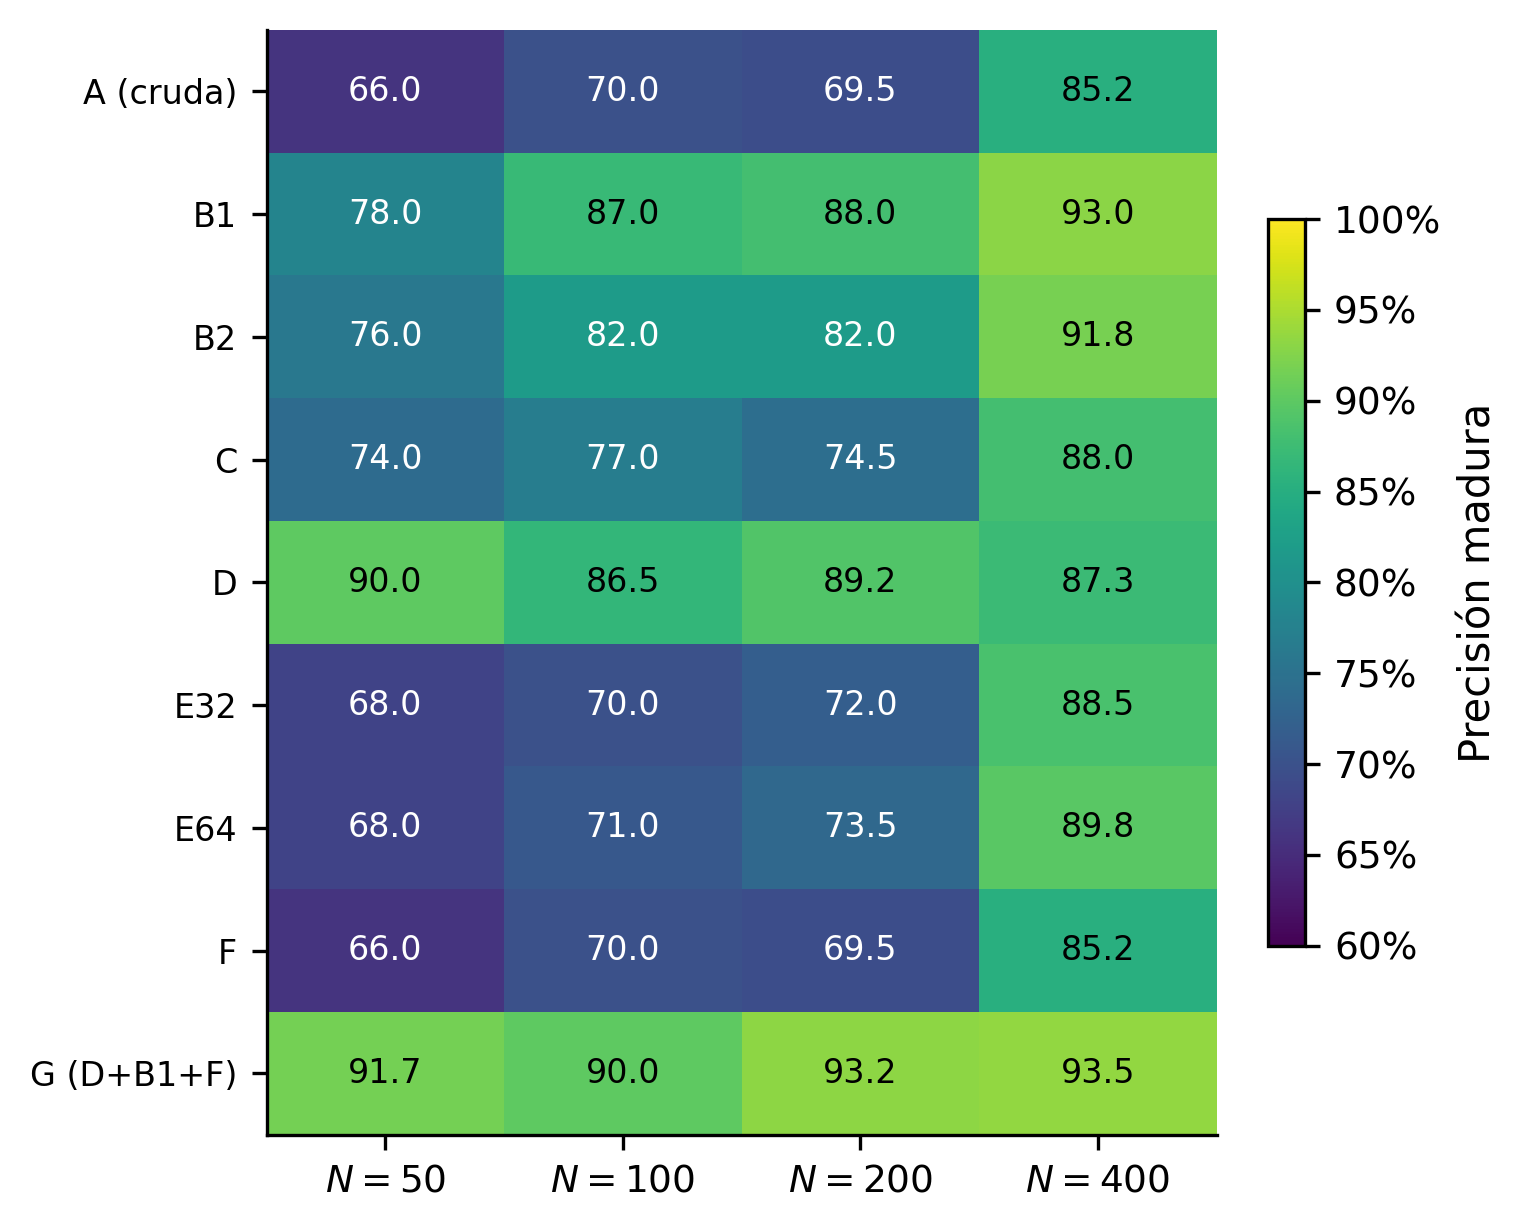
\includegraphics[width=0.75\textwidth]{fig03_heatmap_condition_N.png}
    \caption{Precisión madura (\%) por condición de la Tabla~\ref{tab:calibracion} y
    número de consultas de formación $N$ (mismos datos que la
    Figura~\ref{fig:mature-vs-n}).
    Hasta $N = 200$, A, C, E32, E64 y F quedan entre 66 y 77\%, y B1 sube de 78 a 88\%
    (93\% con $N = 400$); D y G pasan del 86\% en todo el rango.}
    \label{fig:heatmap-condicion}
\end{figure}

\paragraph{Desglose por dominio.}
Con la lectura B1 en $N = 400$, cinco dominios quedan por encima del 90\%
(\texttt{cow}, \texttt{cup} y \texttt{tomato} 100\%, \texttt{car} 98\%, \texttt{dog}
93.9\%) y tres por debajo: \texttt{apple} 88.2\%, \texttt{horse} 88\% y \texttt{pear}
76\% (Figura~\ref{fig:dominio}).
Las clases de fruta comparten léxico genérico (\textit{fruit} las tres, \textit{pome}
\texttt{apple} y \texttt{pear}, \textit{red} \texttt{apple} y \texttt{tomato}) y
concentran 18 de los 28 errores
que deja B1, la mitad \texttt{pear} $\to$ \texttt{apple} (9); el otro foco es
\texttt{horse} $\to$ \texttt{cow} (6).

\begin{figure}[H]
    \centering
    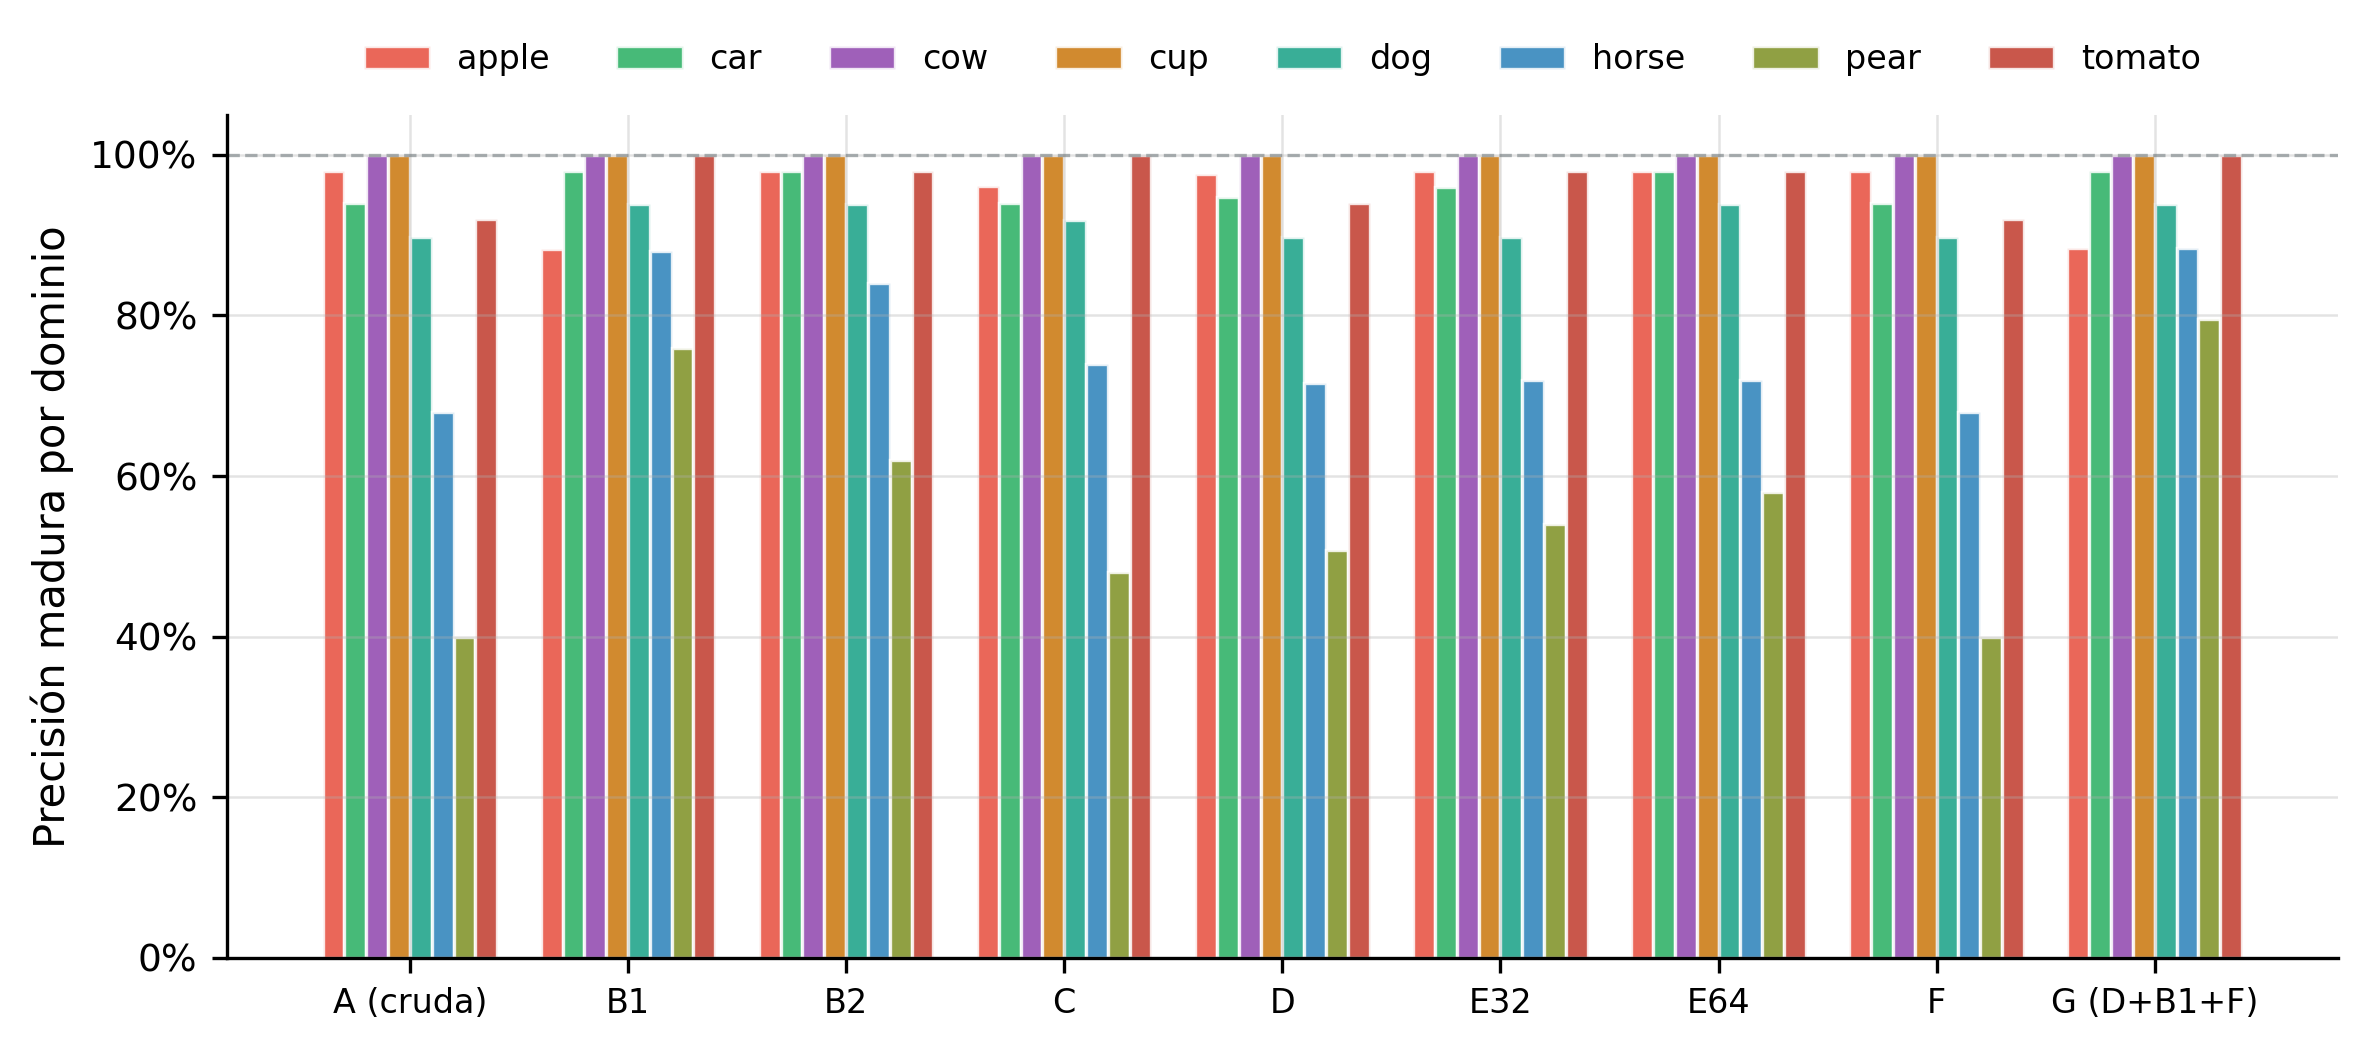
\includegraphics[width=\textwidth]{fig04_domain_accuracy_N400.png}
    \caption{Precisión madura por dominio y condición de la
    Tabla~\ref{tab:calibracion} ($N = 400$, media de 5 semillas).
    \texttt{pear} es el dominio más bajo en todas las condiciones; la lectura B1 lo lleva
    de 40 a 76\% respecto de la cruda (A), y a \texttt{horse} de 68 a 88\%.}
    \label{fig:dominio}
\end{figure}

\paragraph{Con B1, la participación de \texttt{apple} queda cerca del ideal.}
La Figura~\ref{fig:winner} muestra qué fracción de las victorias maduras se lleva cada
módulo.
Con la lectura cruda (A), \texttt{apple} se lleva el 20.5\%: es el sesgo de lectura que
B1 corrige.
Con B1 baja al 13.8\% (ideal 12.5\%), y el módulo que más se aleja del ideal es
\texttt{pear}, a 2.25 puntos (10.25\%).
La Sección~\ref{sec:disc-dominancia} analiza el origen del sesgo.

\begin{figure}[H]
    \centering
    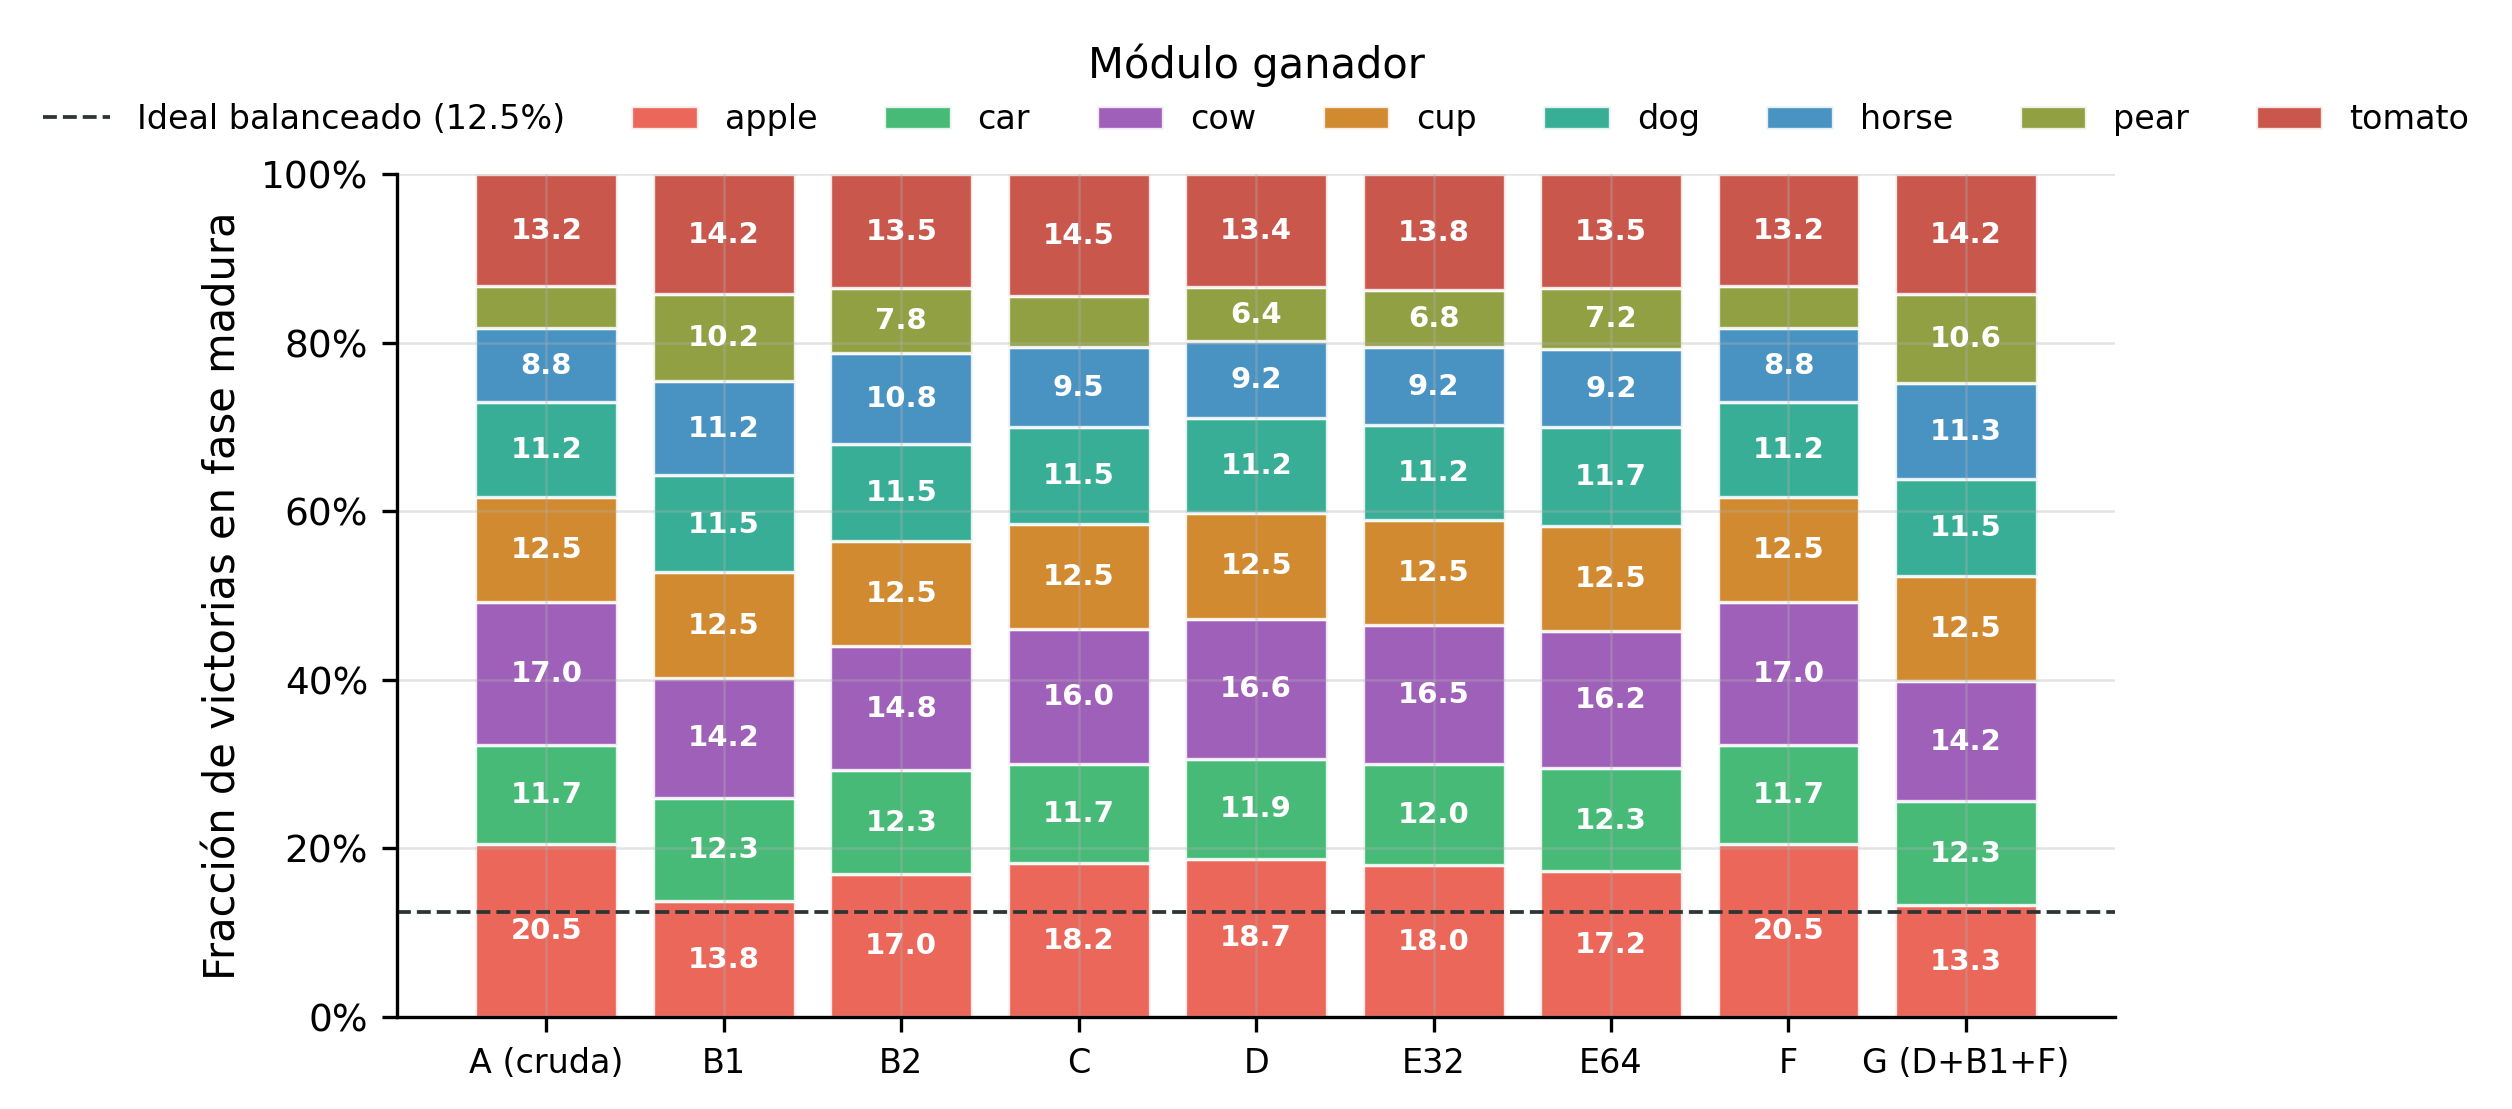
\includegraphics[width=\textwidth]{fig09_winner_distribution_N400.png}
    \caption{Distribución de módulos ganadores en fase madura por condición de la
    Tabla~\ref{tab:calibracion} ($N = 400$, media de 5 semillas; cifras en \%, sin cifra
    en los segmentos menores del 6\%).
    La línea discontinua marca el ideal balanceado de $1/8 = 12.5\%$, con el que se
    compara el segmento inferior (\texttt{apple}).}
    \label{fig:winner}
\end{figure}

\paragraph{Estado del directorio.}
La entropía del directorio transactivo es de 2.974 bits en la condición A y de 2.977 en
G, el 99.1\% del máximo ($\log_2 8 = 3$ bits): los conteos quedan casi parejos entre los
ocho módulos.
El sesgo que B1 corrige está en la lectura, no en los conteos
(Sección~\ref{sec:disc-b1}).

% ---------------------------------------------------------------
\subsection{Protocolo completo}
\label{sec:proto-completo}

El protocolo completo (fase temprana $\to$ formación del directorio $\to$ fase madura
con el TME apagado) se corrió sobre el subconjunto de 80 consultas (10 por clase).
Mide lo mismo que la calibración con el protocolo del sistema, pero el directorio se
forma con 10 consultas por dominio en lugar de unas 50; por eso su precisión madura es
menor que la del banco completo (Sección~\ref{sec:formacion}).

\paragraph{Fase temprana.}
El sistema alcanzó una precisión temprana del 81.2\% con una tasa de rechazo del 5.0\%;
los rechazos los decide la memoria, sin filtro de vocabulario
(Sección~\ref{sec:pipeline-semantico}).

\paragraph{Fase madura.}
Con la lectura B1, la precisión madura fue del 81.2\% y la fidelidad temprana-madura del
92.5\%; con la lectura cruda, la precisión madura baja al 72.5\%.
El directorio terminó con los conteos $[46, 16, 40, 25, 30, 18, 21, 31]$ para
(\texttt{apple}, \texttt{car}, \texttt{cow}, \texttt{cup}, \texttt{dog}, \texttt{horse},
\texttt{pear}, \texttt{tomato}) y una entropía de 2.914 bits sobre un máximo de 3.000.

\paragraph{Réplica con las 16 consultas de referencia.}
Con las 16 consultas de referencia del sistema (\texttt{TEST\_QUERIES}, 2 por dominio),
el enrutamiento acierta 15 de 16, con al menos un acierto en cada clase y conteos
$[12, 6, 6, 7, 5, 5, 4, 7]$;
el único error es una consulta de fruta con léxico compartido
(``a ripe green pear from the orchard'' $\to$ \texttt{apple}).

\paragraph{Sonda de rechazo fuera de dominio.}
Aparte del banco, se presentaron 12 consultas \emph{representables} (todas tienen vector
fastText) que describen objetos fuera de los ocho dominios.
La memoria rechazó 10 de 12 por contención (puntuación cero en los ocho módulos).
Las 2 restantes se enrutan porque comparten tokens con etiquetas legítimas de algún
dominio (p.\ ej.\ \textit{food}): la frontera entre ``fuera de dominio'' y ``comparte
conceptos con el dominio'' es semántica, no léxica.

% ---------------------------------------------------------------
\subsection[Parámetros nativos iota x kappa]{Parámetros nativos $\iota \times \kappa$}
\label{sec:param-iota-kappa}

Los dos parámetros propios de la EAM (Sección~\ref{sec:eam}) son la poda $\iota$, que
apaga durante la recuperación las celdas de peso menor que $\iota$ veces el peso medio
de las celdas no nulas, y el umbral relativo $\kappa$, que exige a la activación media
por celda de la proyección llegar a $\kappa$ veces la media de la memoria.
La pregunta es si alguno mejora la fase temprana o hace innecesaria la normalización B1.
Se barrió una cuadrícula con $\iota \in \{0, 0.25, 0.5, 1.0\}$ y siete valores de
$\kappa$: 0 y los cuantiles 10, 25, 50, 75, 90 y 100\,\% de esa razón, medida con
$\iota = 0$ sobre los 260 pares (token, módulo) del subconjunto de 80 consultas en que el
módulo contiene al token, lo que da
$\kappa \in \{0, 1.755, 1.801, 1.844, 1.937, 2.056, 2.107\}$.
La Tabla~\ref{tab:grid-iota-kappa} muestra la precisión temprana y el rechazo.

\begin{table}[H]
    \centering
    \caption{Precisión temprana y, entre paréntesis, tasa de rechazo (\%) en función de
    $\iota$ y $\kappa$ (80 consultas). Con $\iota \geq 0.25$ el valor no cambia con
    $\kappa$: la poda sube la razón que $\kappa$ compara por encima del mayor $\kappa$
    del barrido.}
    \label{tab:grid-iota-kappa}
    \small
    \begin{tabular}{cccccccc}
        \toprule
        & \multicolumn{7}{c}{$\kappa$} \\
        \cmidrule(lr){2-8}
        $\iota$ & 0 & 1.755 & 1.801 & 1.844 & 1.937 & 2.056 & 2.107 \\
        \midrule
        0.00 & 81.2 (5.0) & 77.5 (6.2) & 65.0 (10.0) & 57.5 (18.8) & 35.0 (45.0) & 18.8 (63.8) & 0.0 (100.0) \\
        0.25 & 82.5 (5.0)  & \multicolumn{6}{c}{igual en todas las columnas} \\
        0.50 & 75.0 (11.2) & \multicolumn{6}{c}{igual en todas las columnas} \\
        1.00 &  8.8 (86.2) & \multicolumn{6}{c}{igual en todas las columnas} \\
        \bottomrule
    \end{tabular}
\end{table}

\paragraph{Efecto de $\iota$.}
Una poda ligera ($\iota = 0.25$) quita algo de ruido de baja frecuencia: la fase
temprana pasa de 81.2 a 82.5\% y la madura con B1 de 81.2 a 83.8\% (la
Tabla~\ref{tab:grid-iota-kappa} solo da la fase temprana).
Una poda mayor destruye: $\iota = 0.5$ pierde 6 puntos con un rechazo del 11\%, y
$\iota = 1.0$ rechaza el 86\%.
La poda elimina conocimiento escaso pero válido antes de eliminar relaciones espurias.

\paragraph{Efecto de $\kappa$.}
Con $\iota = 0$, $\kappa$ solo rechaza: a medida que sube, la precisión baja de 81.2\%
a 0.0\% y el rechazo sube de 5.0\% a 100\%, y ninguna columna mejora la línea base.
El umbral relativo descarta por igual pistas válidas y espurias, porque la razón que
compara (entre 1.52 y 2.11) no separa a unas de otras.
Con $\iota \geq 0.25$, $\kappa$ no actúa en este rango: la poda concentra la activación
en las celdas que sobreviven y la media de la memoria no cambia, así que la razón
mínima sube a 2.33, 2.79 y 3.96, por encima del $\kappa$ máximo.
$\kappa$ no es una defensa contra el sesgo de masa.

\paragraph{Ninguna condición nativa sustituye a B1.}
En las dos condiciones nativas llevadas hasta la fase madura, la lectura cruda queda por
debajo de B1: 72.5\% frente a 81.2\% en la línea base y 80.0\% frente a 83.8\% en la
mejor condición nativa ($\iota = 0.25$, $\kappa = 0$).
También se probó dividir la puntuación temprana de cada módulo entre la media de su
memoria de contenido ($\div$\texttt{mem.mean}): \emph{empeora} la fase temprana (76.2\%)
y distorsiona los conteos del directorio, porque con el llenado por instancias las masas
de contenido ya están igualadas por construcción y esa corrección sobra.

% ---------------------------------------------------------------
\subsection{Formación del directorio transactivo}
\label{sec:formacion}

Se midió cuántas interacciones necesita el directorio para volverse utilizable y si
importa su orden: tras cada interacción $t$ de la fase temprana se evaluó la precisión
madura (lectura B1) sobre las 80 consultas, con el directorio tal como estaba en ese
momento, en cuatro condiciones: orden intercalado entre dominios, barajado (5 semillas),
bloqueado por dominio (todas las consultas de una clase y luego las de la siguiente) y
un control en orden intercalado que elige al ganador temprano con la puntuación cruda,
sin compuerta ni normalización.

\paragraph{Con 10 consultas por clase, ninguna condición llega al 90\%.}
Todas convergen al 81.2\% final.
Con ocho dominios y consultas que comparten léxico, 10 interacciones por dominio no
acumulan suficiente evidencia distintiva; el mismo protocolo con el banco completo
alcanza el 93.0\% (Sección~\ref{sec:calibracion}).

\paragraph{El orden afecta la velocidad, no el destino.}
Las cuatro condiciones terminan en el mismo estado: los conteos y la entropía de la
Sección~\ref{sec:proto-completo} (2.914 bits).
El orden sí cambia la velocidad: la precisión madura llega al 70\% tras 13 interacciones
en orden intercalado, tras 28 a 42 en orden barajado (según la semilla) y tras 59 en
orden bloqueado; al 75\%, tras 18, 40 a 51 y 71.
Esta invariancia del destino muestra que el directorio acumula evidencia conmutativa:
el orden solo determina cuándo se vuelve utilizable, no qué se aprende.

% ---------------------------------------------------------------
\subsection{Capacidad de llenado}
\label{sec:capacidad}

Se varió el número de imágenes registradas por clase,
$N \in \{25, 50, 100, 200, 328\}$, con el llenado imagen por imagen
(\textit{imagen--etiqueta}).
Una imagen se acepta si la memoria del módulo la contiene desde el lado de la imagen
(contención inversa, con $\xi = 0$); los \textit{falsos} se miden con imágenes de otras
clases presentadas al módulo.
La Tabla~\ref{tab:capacidad} resume las métricas.

\begin{table}[H]
    \centering
    \caption{Métricas de capacidad en función del número de imágenes registradas $N$
    por clase.
    ``Llenado propio'' y ``Prueba propia'': fracción de imágenes de la propia clase, de
    llenado y de prueba, que el módulo acepta; ``Falsos'': fracción de imágenes de otras
    clases que acepta.
    ``Enrutamiento'' es la precisión temprana sobre 80 consultas (reconocimiento por el
    contenido llenado con $N$ imágenes, sin directorio); ``Variedad $L_1$'' es la
    distancia media $L_1$ entre recuperaciones de una misma pista; $H$ es la entropía de
    la memoria de contenido.}
    \label{tab:capacidad}
    \small
    \setlength{\tabcolsep}{4pt}
    \begin{tabular}{ccccccc}
        \toprule
        $N$ & Llenado propio (\%) & Prueba propia (\%) & Falsos (\%) & Variedad $L_1$ & Enrutamiento (\%) & $H$ (bits) \\
        \midrule
         25  & 100 &  0 & 0 & 1.90 & 61.3 & 3.648 \\
         50  & 100 &  0 & 0 & 1.86 & 72.5 & 4.369 \\
        100  & 100 &  2 & 0 & 1.74 & 78.8 & 4.950 \\
        200  & 100 & 20 & 0 & 1.91 & 81.2 & 5.204 \\
        328  & 100 & 56 & 0 & 2.18 & 81.2 & 5.318 \\
        \bottomrule
    \end{tabular}
\end{table}

\paragraph{Generalización con el volumen de llenado.}
Con $\xi = 0$ el sistema no generaliza desde cero; la generalización a imágenes de prueba
aparece a medida que el llenado cubre más del espacio latente de la clase (del 0\% en
$N = 25$ al 56\% en $N = 328$), sin necesidad de ajustar $\xi > 0$ en el contenido.

\paragraph{Especificidad.}
Con el llenado de un latente por imagen, la tasa de falsos aceptados es del 0\% en todo
el rango de $N$ probado, con siete clases contrarias por módulo.

\paragraph{Enrutamiento y entropía.}
La precisión temprana crece con $N$ y se estabiliza en torno al 81\% desde $N = 200$; la
entropía de la memoria de contenido crece con $N$ y se satura (3.65, 4.37, 4.95, 5.20 y
5.32 bits), coherente con la acumulación de variedad.
El sistema opera con $N = 200$: ahí la precisión temprana ya se estabilizó, y quedan
\texttt{train[200:328]} para las interacciones visuales (Sección~\ref{sec:dataset}).

% ---------------------------------------------------------------
\subsection{Hemisferio visual}
\label{sec:hemisferio-visual}

El hemisferio visual opera en dos fases: formación (registro de percepciones reales de
\texttt{train[200:328]} en los directorios visuales) y evaluación (enrutamiento de las
656 imágenes de prueba mediante el directorio visual por módulo).

\paragraph{Fase A: formación con 1024 imágenes.}
Se presentaron 1024 imágenes (128 por clase) en orden intercalado.
Sobre las percepciones aceptadas, el enrutamiento visual acertó el 99.9\%, con un
rechazo del 0.8\% y una percepción rechazada antes de la memoria por el umbral de
energía.
Cada percepción aceptada registra sus 16 variantes; el registro completo del TME quedó
en $[2048, 2016, 2016, 2016, 2016, 2032, 2048, 2048]$, con entropía de 3.000 bits al
tercer decimal, el máximo con ocho módulos.
Los directorios visuales de cada módulo quedan entre 2.22 y 2.41 bits, con 2016--2048
registros propios contra 144--368 de cada otro módulo, como corresponde a un registro
perspectival.

\paragraph{Fase B: enrutamiento de imágenes de prueba.}
Las 656 imágenes de prueba se enrutaron mediante los directorios visuales por módulo
($M^R_{\mathrm{dir}}$) con lectura B1 estricta ($\xi = 0$, directorios perspectivales):
cada imagen entra por un módulo no especialista, que la redirige o la rechaza.
El resultado fue de 631 de 656 imágenes (96.2\%) asignadas correctamente, 23 rechazadas
(3.5\%; cuatro de ellas antes de la memoria, por el umbral de energía) y dos falsos
enrutamientos (0.3\%); sobre las aceptadas, la precisión es del 99.7\%.

\paragraph{Más variantes, más cobertura.}
El directorio visual no tolera huecos ($\xi = 0$; la razón está en la
Sección~\ref{sec:operaciones}): con $\xi = 2$, el enrutamiento del dominio propio baja a
medida que el módulo presencia más dominios ajenos (experimento 10).
La palanca para la cobertura es densificar el llenado, no tolerar huecos.
El experimento 13 lo mide sobre las 656 imágenes de prueba: registrar en el directorio 16
variantes por percepción, en lugar de una, lleva su aceptación del 73.6 al 96.2\,\% (con
4 variantes, 87.7\,\%); con 16 variantes también en el contenido, la \emph{cobertura de
punta a punta} (imágenes enrutadas a su clase cuyo destino además responde) pasa de 66.5
a 94.5\,\%, y el rechazo de la fase A baja del 4.2 al 0.8\,\%.
En ese experimento, con una o 4 variantes en el directorio no hay enrutamientos falsos y
con 16 hay uno; el sistema, con sus 16 variantes, enruta mal dos de las 656 imágenes
(Sección~\ref{sec:limitaciones}).

\paragraph{Evocación de dominio: imagen $\to$ palabras.}
Sobre las primeras 15 imágenes de prueba de cada clase que el enrutamiento acepta (116 de
120), la evocación inversa desde el módulo destino (recuperación $\beta$ desde el
latente, decodificada por similitud coseno top-3) produjo al menos una etiqueta del
vocabulario de la clase real en 113 de 116 (97.4\%) de los casos.

\paragraph{El rechazo y la salida semántica los decide la memoria.}
Reconocimiento, rechazo y reconstrucción son operaciones de la propia memoria: el
codificador ResNet18 solo convierte la imagen en una pista latente, y a partir de ahí la
EAM decide.
La Figura~\ref{fig:rechazo-imagenes} ilustra el rechazo: imágenes reales que la memoria
contiene se aceptan, mientras que imágenes reales no contenidas y las sondas sintéticas
de ruido y de píxeles barajados reciben puntuación cero en los ocho módulos y se
rechazan, sin que intervenga ningún filtro externo.
La tercera sonda, un lienzo gris uniforme, no llega a la memoria: la norma de su
latente (10.7) queda por debajo del umbral de energía $\tau = 16.61$
(Sección~\ref{sec:percepcion}), igual que una vista real de \texttt{cow} del panel.
Sin ese umbral, el contenido sí le daría soporte. El experimento 14 localizó la causa:
el codificador lleva las entradas sin estructura (gris uniforme, un objeto desenfocado o sin
contraste) a latentes de norma baja que caen dentro de la envolvente por coordenada de
los animales. Los grises de nivel 120 a 160 (el del panel, 127, cae en ese tramo) los
aceptan a la vez \texttt{cow}, \texttt{dog} y \texttt{horse}, aunque la instancia real
más cercana está a entre 2.4 y 2.9 veces la mediana de la distancia intraclase.
No es cualquier fondo liso: de 12 sólidos de color se aceptan 2.
Esos grises tienen norma de 10.7 a 13.0, y el umbral los rechaza.
Las entradas degeneradas que sí pasan el umbral se discuten en la
Sección~\ref{sec:limitaciones}.
La Figura~\ref{fig:imagen-etiquetas} muestra la salida semántica: para cada imagen
aceptada, la reconstrucción es lo que la memoria \emph{evoca} (decodificación de la
recuperación desde la lectura latente $M^R$), no la imagen de entrada, y el sistema devuelve
las etiquetas asociadas.
Que la reconstrucción difiera de la entrada es esperado y honesto: refleja que decide
la distribución acumulada en la memoria.

\begin{figure}[H]
    \centering
    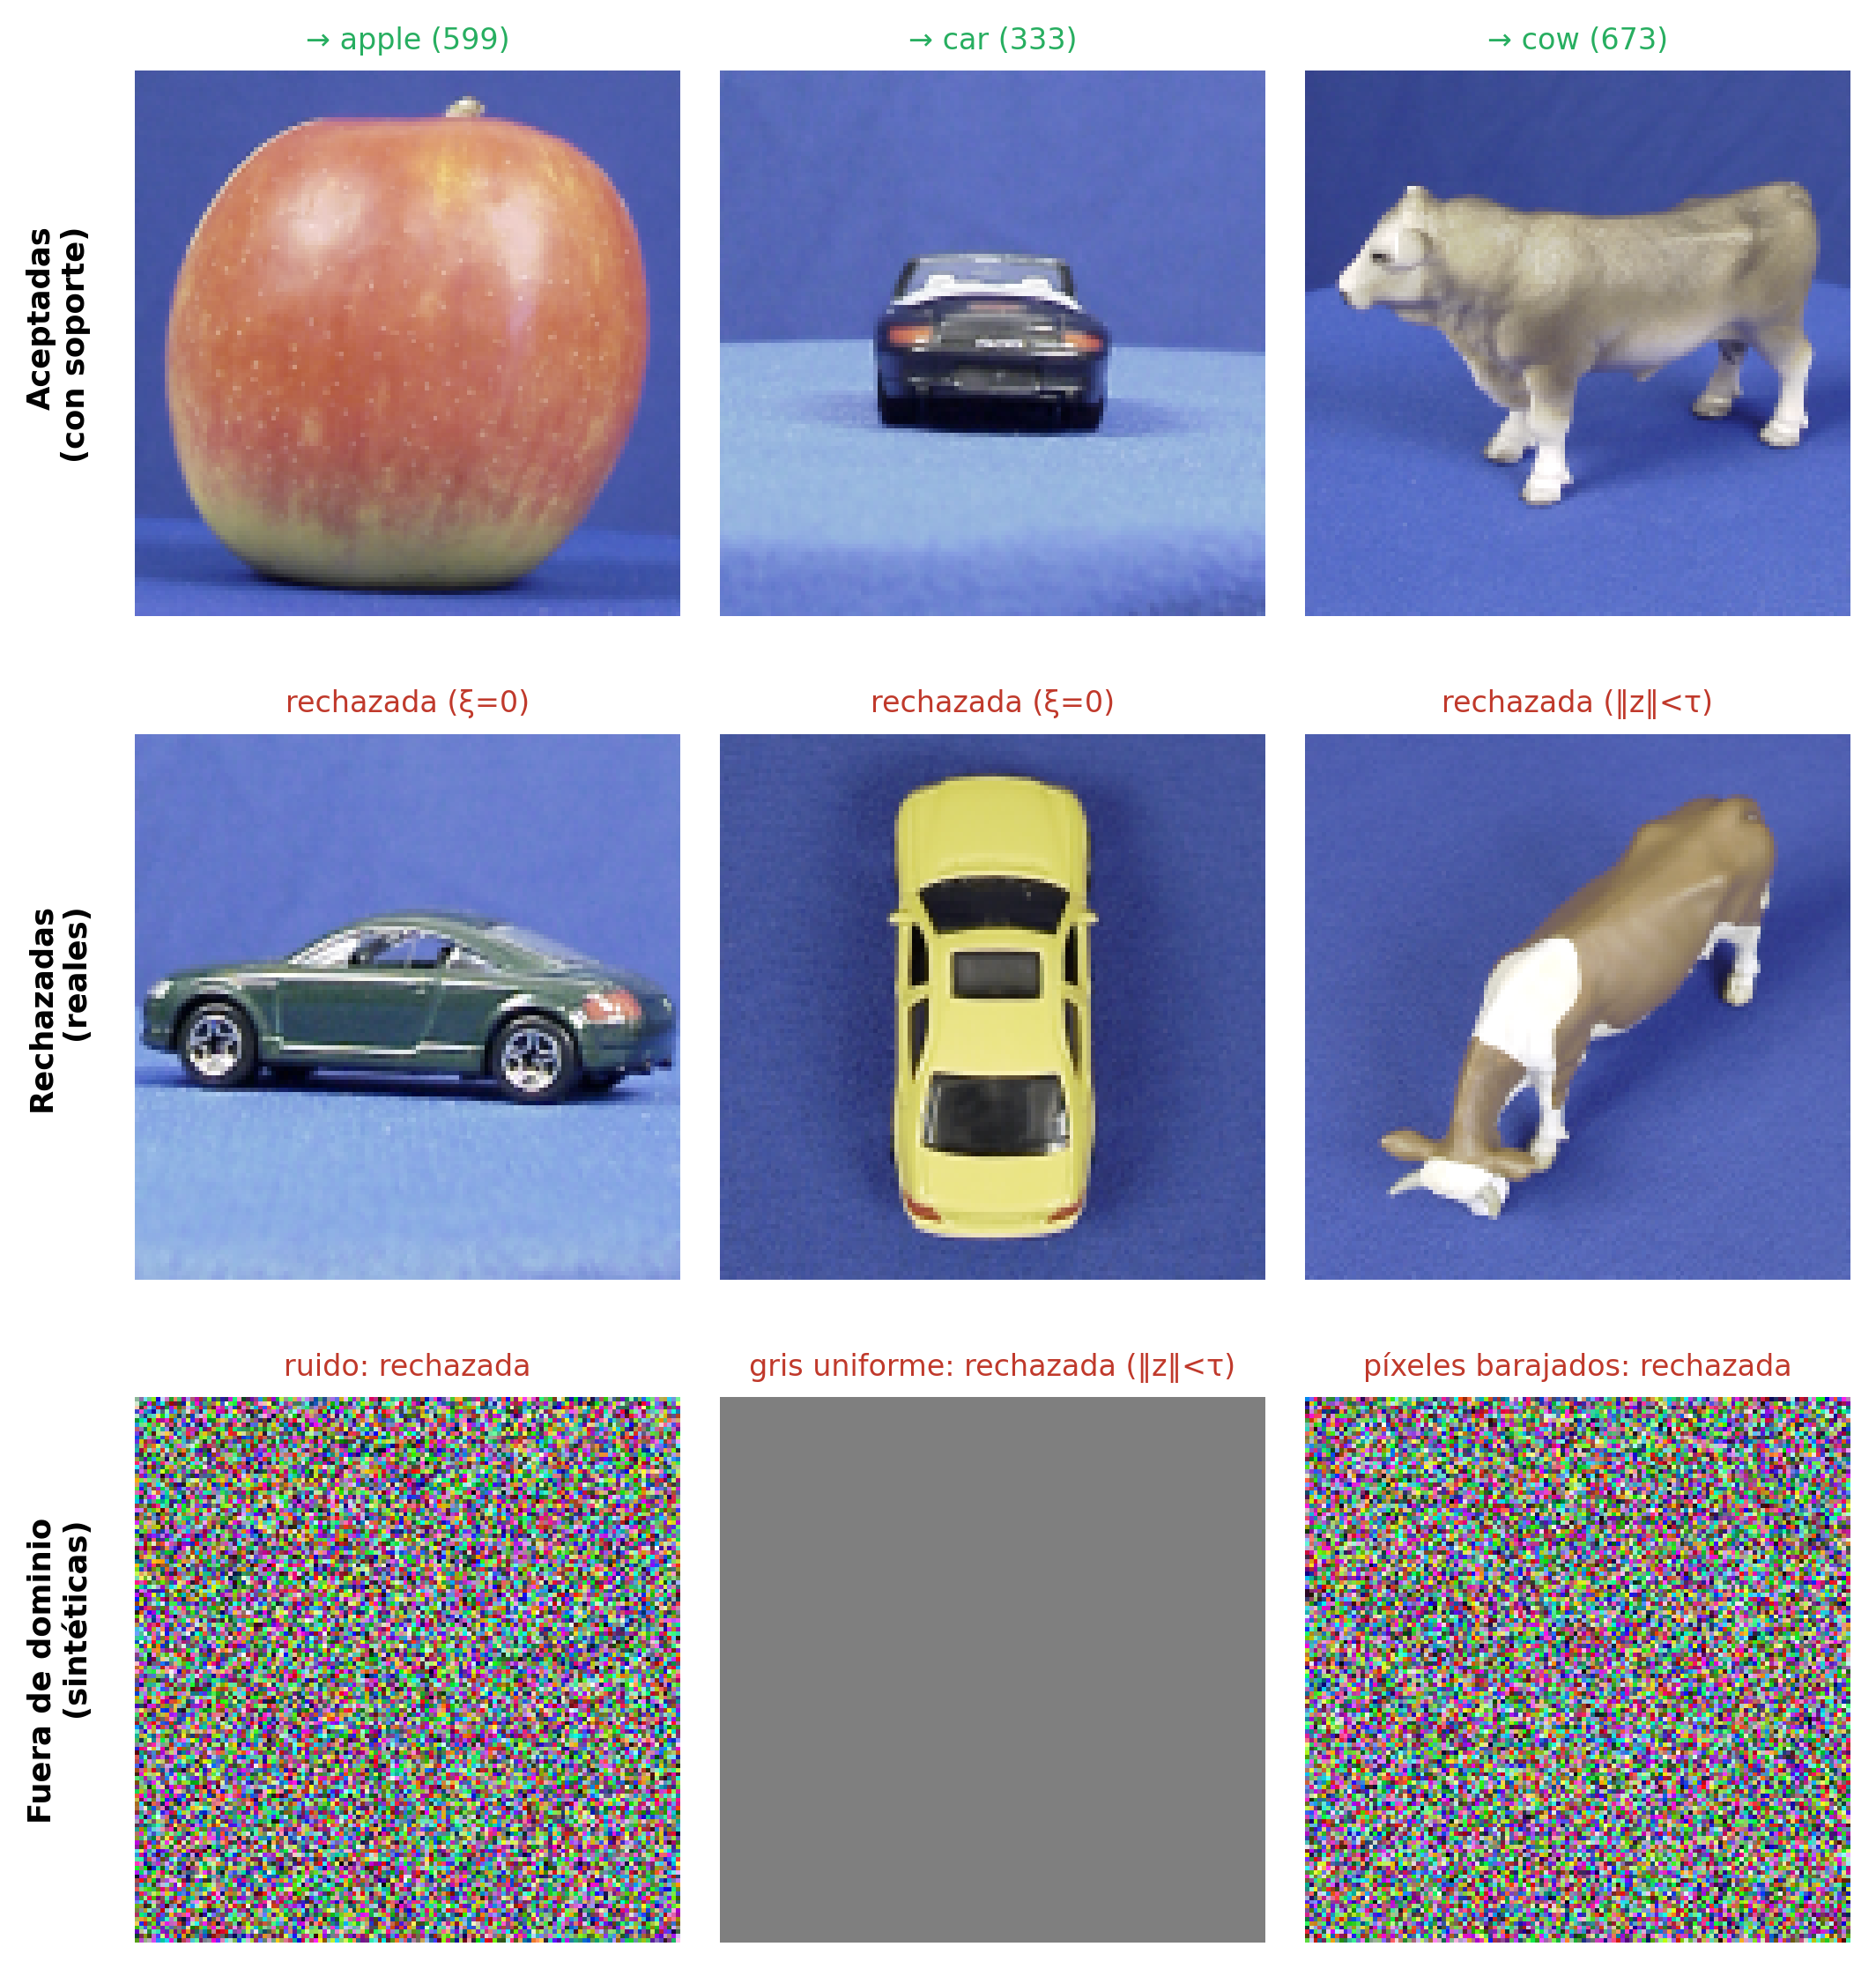
\includegraphics[width=0.85\textwidth]{fig15_image_rejection.png}
    \caption{Rechazo de imágenes en el hemisferio visual (sin filtro léxico), con el umbral
    de energía $\tau$ y la contención en el mismo orden que el sistema. Arriba: imágenes de
    prueba aceptadas por el contenido, con el módulo de mayor soporte y su puntuación de
    contención. En medio: imágenes de prueba rechazadas, dos porque ningún módulo las
    contiene ($\xi = 0$) y una vista de \texttt{cow} porque la norma de su latente no
    alcanza $\tau$. Abajo: sondas sintéticas; el ruido y los píxeles barajados reciben
    puntuación cero en los ocho módulos, y el gris uniforme se rechaza antes de la memoria
    por el umbral $\tau$.}
    \label{fig:rechazo-imagenes}
\end{figure}

\begin{figure}[p]
    \centering
    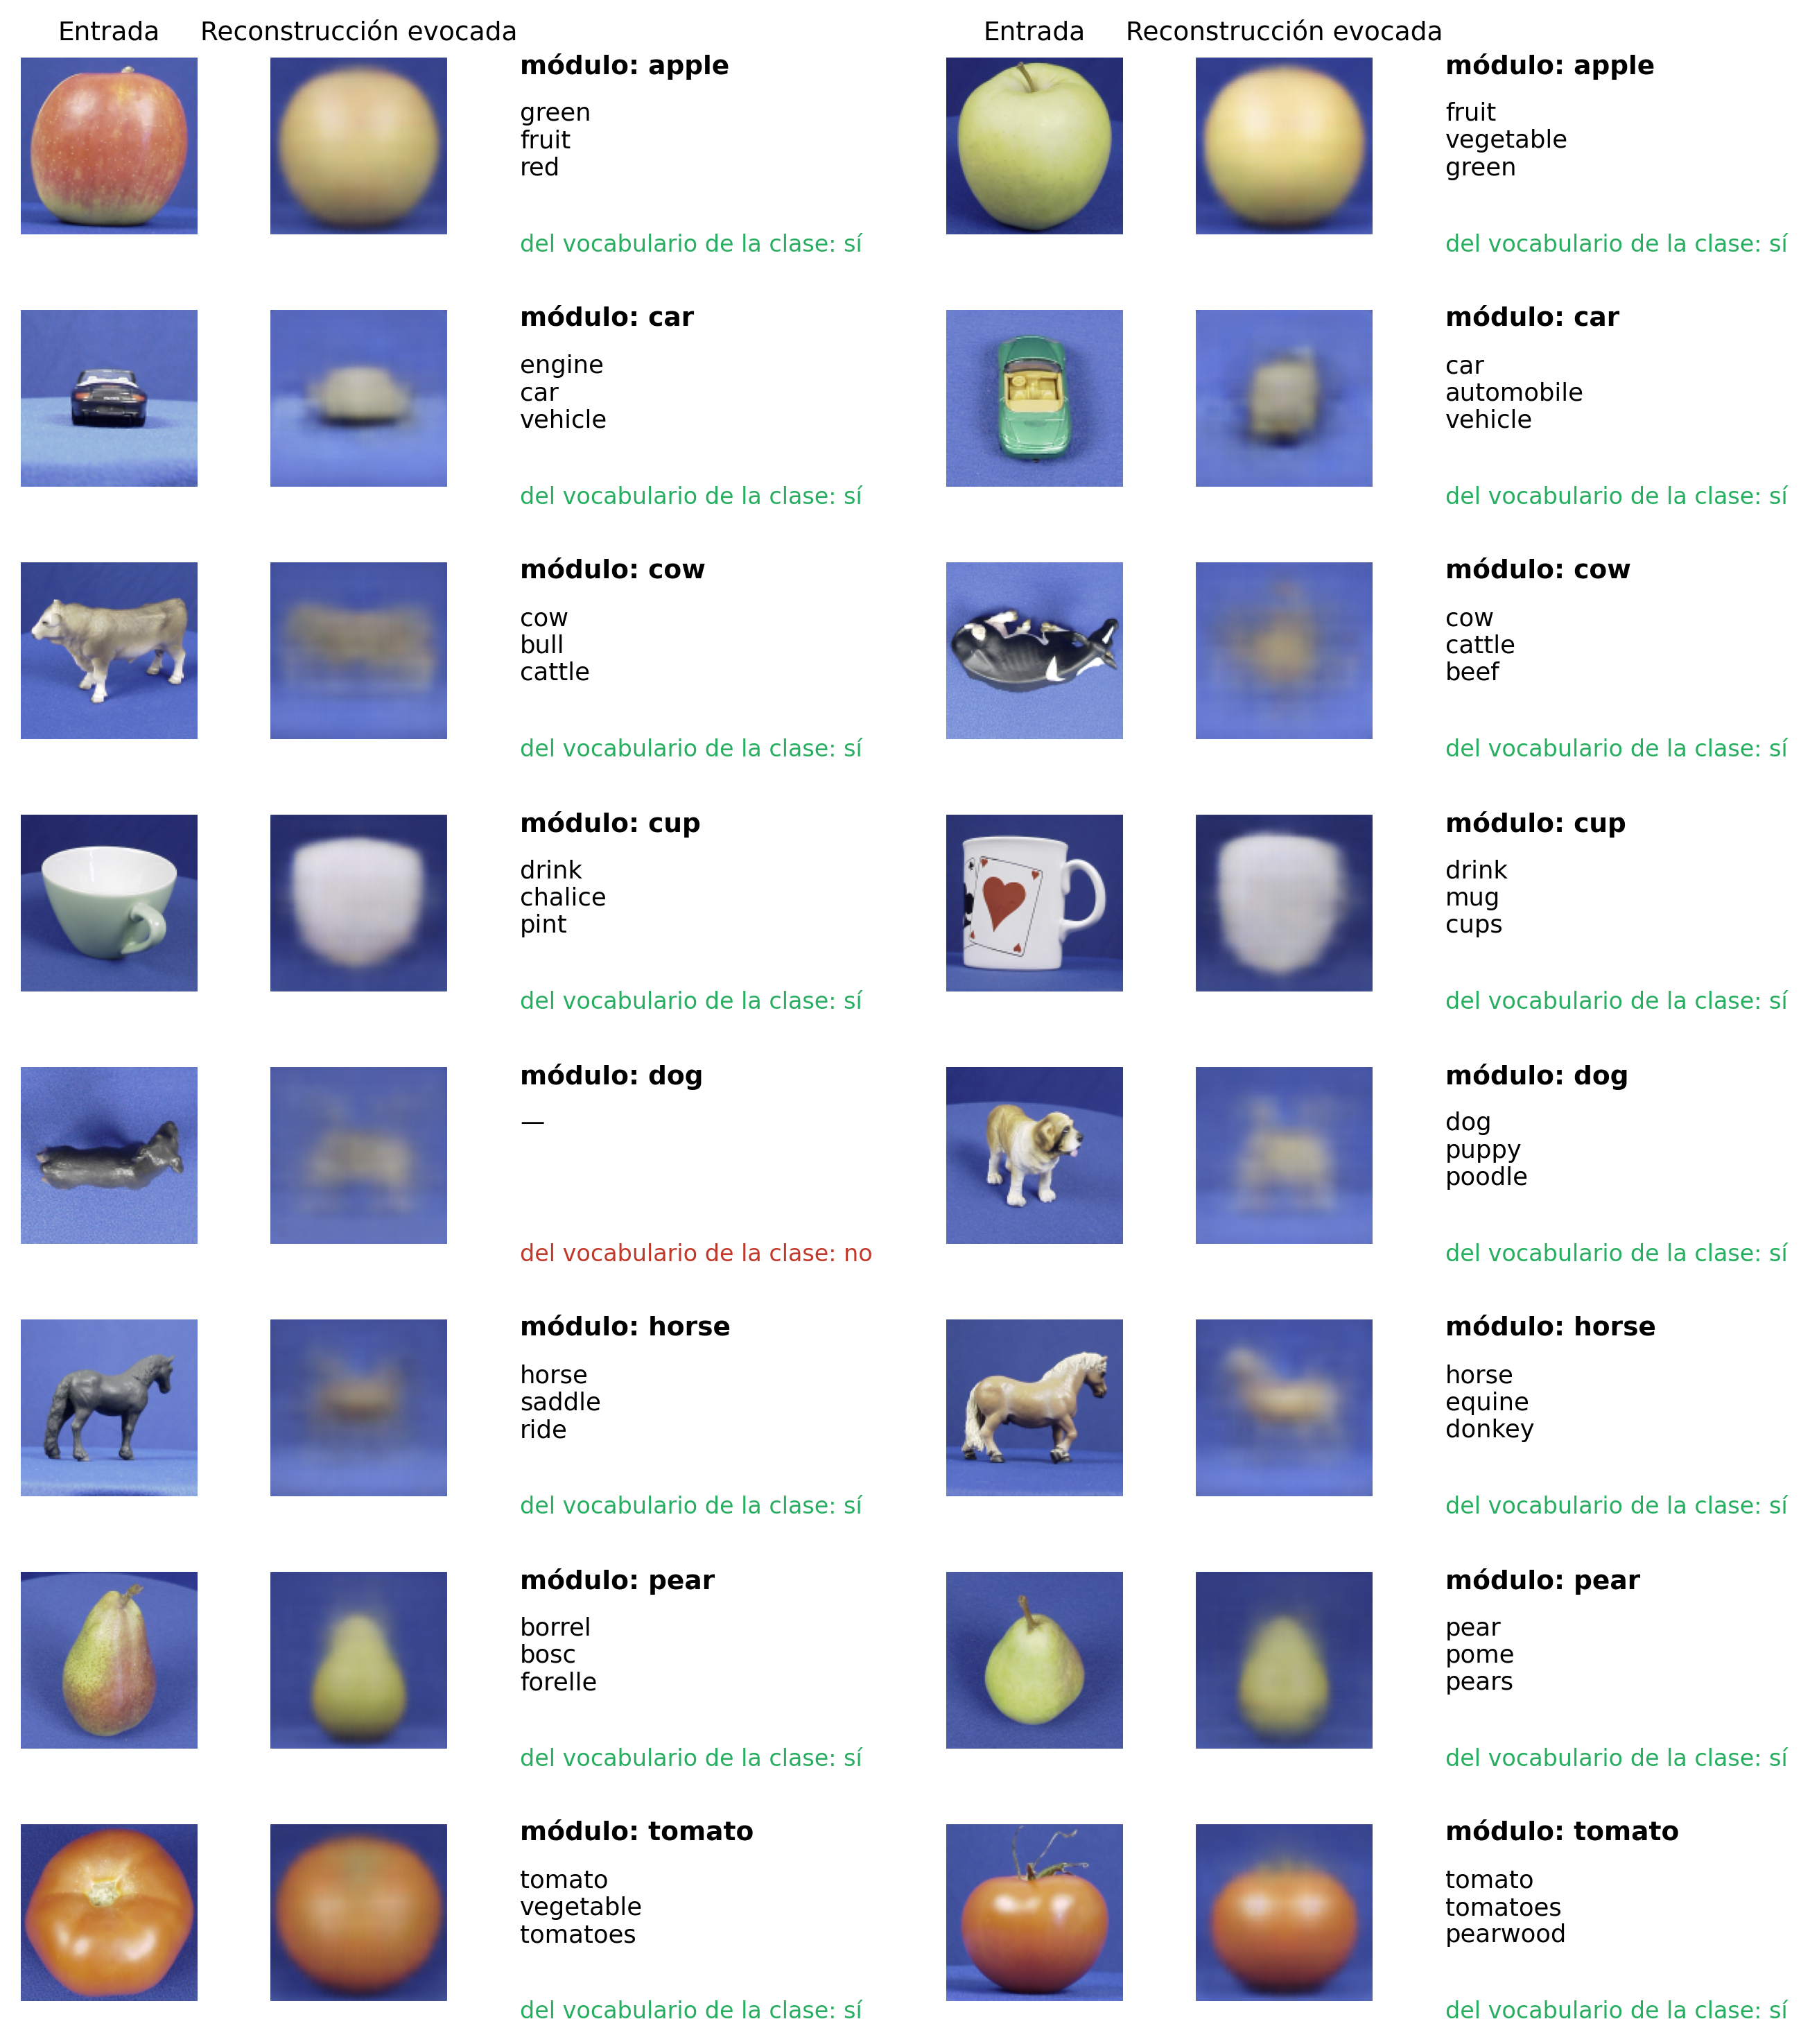
\includegraphics[width=\textwidth]{fig16_image_to_labels.png}
    \caption{Salida semántica imagen $\to$ etiquetas: las dos primeras imágenes de prueba
    de cada clase que pasan el umbral de energía y que algún módulo contiene (el de mayor
    soporte, sin pasar por el directorio).
    Por imagen: la entrada, la reconstrucción que evoca la memoria (no la entrada) y las
    tres etiquetas recuperadas, con la marca de si alguna es del vocabulario de la clase
    real.
    En 15 de los 16 ejemplos alguna etiqueta es del dominio; en el restante
    (\texttt{dog}) la recuperación no devuelve etiquetas.
    Con el directorio, sobre las primeras 15 imágenes de prueba de cada clase que el
    enrutamiento acepta (116), la evocación acierta el 97.4\% (113).}
    \label{fig:imagen-etiquetas}
\end{figure}

% ---------------------------------------------------------------
\subsection{Generalización a objetos nuevos}
\label{sec:objetos-nuevos}

La partición principal separa imágenes, no objetos: los diez objetos de cada clase
aportan vistas al llenado y a la prueba (Sección~\ref{sec:dataset}), así que las cifras
anteriores miden vistas nuevas de objetos conocidos.
La generalización a objetos nuevos se midió aparte (experimento 16), con una validación
\textit{leave-one-object-out} de diez pliegues: en cada pliegue, el contenido y la fase A
se construyen con nueve objetos por clase, y sobre los mismos modelos se evalúan las 41
vistas del objeto reservado de cada clase y 41 vistas no usadas de los objetos que sí
contribuyeron.
La cobertura de punta a punta es del 89.2\,\% [85.1, 93.2] con objetos nuevos y del
95.5\,\% [95.1, 95.9] con objetos conocidos; la brecha es de 6.3 puntos [2.5, 10.4]
(intervalos de 95\,\% por remuestreo de los pliegues).
El enrutamiento correcto sobre las imágenes aceptadas es del 99.9\,\% en los dos bancos,
y los falsos enrutamientos con objetos nuevos son 2 de 3280 (un \texttt{cow} y un
\texttt{horse}, enviados a \texttt{dog}): la envolvente por coordenada cubre a un objeto
que no contribuyó a ella, y cuando no lo cubre lo rechaza.
La brecha no se reparte entre clases sino que se concentra en objetos concretos: 71 de
los 80 objetos reservados superan el 70\,\%, y nueve (dos manzanas, dos peras, dos
perros, una taza, un coche y una vaca) concentran el 57\,\% de los fallos.

% ---------------------------------------------------------------
\subsection{Línea base: una sola EHAM con las ocho clases}
\label{sec:eham-unica}

Esta sección mide qué aporta repartir el contenido entre ocho especialistas frente a
guardarlo todo en una sola memoria.
Se construyó una EHAM única con los mismos pares etiqueta--latente que reciben los ocho
especialistas (25\,600 con 200 imágenes por clase y 16 variantes) y se evaluó con las
mismas operaciones de reconocimiento con compuerta y de recuerdo desde la etiqueta
(\texttt{recognize\_gated}, \texttt{recall\_from\_left}), sin enrutamiento.
Se compararon tres brazos: la \emph{EHAM única}; los especialistas con el módulo elegido
por la verdad de terreno (\emph{oráculo}, un techo), y el \emph{protocolo} transactivo
completo, que elige el módulo con el directorio.
Las consultas de texto son las 171 del banco que no se usaron para formar los
directorios (las otras 240 los forman); las de imagen, las primeras 10 imágenes de
prueba de cada clase.
Se corrieron 10 semillas con 25, 50, 100 y 200 imágenes por clase.
Cada recuerdo se juzga por la clase de la instancia real más cercana (juez 1-NN) y por
la distancia a ella.
Con 200 imágenes por clase, cuatro de los ocho especialistas reconstruidos son idénticos
bit a bit a las memorias del sistema; los otros cuatro difieren porque el experimento
recalcula los latentes en GPU, y el redondeo puede mover un registro al nivel vecino.
La Tabla~\ref{tab:eham-unica} resume los resultados; las tablas completas, con sus
intervalos, están en \texttt{results/experimento11/}.

\begin{table}[H]
    \centering
    \caption{Una sola EHAM contra los especialistas, por número de imágenes de llenado
    por clase (media de 10 semillas). Texto: 171 consultas reservadas; clase correcta
    según el juez 1-NN, distancia a la instancia real más cercana y, en el protocolo,
    enrutamiento a la clase de la consulta. Imagen $\to$ texto: 80 imágenes de prueba;
    fracción respondida y fracción respondida con el dominio de otra clase. Fuera de
    dominio: consultas aceptadas de 40; entre paréntesis, con la doble compuerta de
    contenido.}
    \label{tab:eham-unica}
    \small
    \begin{tabular}{llcccc}
        \toprule
        & & \multicolumn{4}{c}{Imágenes por clase} \\
        \cmidrule(lr){3-6}
        Medida & Brazo & 25 & 50 & 100 & 200 \\
        \midrule
        Clase correcta (\%)        & EHAM única & 97.6 & 97.5 & 97.6 & 96.9 \\
                                   & Protocolo  & 96.9 & 98.8 & 98.8 & 98.3 \\
                                   & Oráculo    & 100  & 100  & 100  & 100  \\
        \midrule
        Enrutamiento correcto (\%) & Protocolo  & 95.3 & 97.4 & 97.4 & 97.0 \\
        \midrule
        Distancia a la instancia   & EHAM única & 22.9 & 26.6 & 29.4 & 32.5 \\
        real más cercana           & Protocolo  & 19.0 & 20.7 & 23.8 & 27.0 \\
                                   & Oráculo    & 18.2 & 20.4 & 23.3 & 26.8 \\
        \midrule
        Imagen $\to$ texto:        & EHAM única & 78.7 & 95.0 & 98.8 & 100  \\
        responde (\%)              & Oráculo    & 43.8 & 75.0 & 92.5 & 97.5 \\
                                   & Protocolo  & 41.2 & 67.5 & 78.7 & 81.2 \\
        \midrule
        Imagen $\to$ texto:        & EHAM única & 5.5  & 7.5  & 10.5 & 10.9 \\
        dominio ajeno (\%)         & Oráculo    & 0.1  & 1.9  & 2.6  & 4.1  \\
                                   & Protocolo  & 0.2  & 1.8  & 2.2  & 3.0  \\
        \midrule
        Fuera de dominio           & EHAM única & 2     & 2     & 5     & 8     \\
        aceptadas (de 40)          & Protocolo  & 4 (2) & 4 (2) & 4 (2) & 4 (2) \\
                                   & Oráculo    & 2     & 2     & 2     & 2     \\
        \bottomrule
    \end{tabular}
\end{table}

\paragraph{Acierto de clase.}
Con 25 imágenes por clase la EHAM única acierta la clase algo más que el protocolo
(97.6\,\% frente a 96.9\,\%), con intervalos de 95\,\% que se solapan ($[97.4, 97.8]$ y
$[96.3, 97.6]$).
Desde 50 el orden se invierte y los intervalos se separan (con 200, $[97.9, 98.6]$ para
el protocolo y $[96.7, 97.1]$ para la EHAM única).
Lo que cuesta elegir el módulo con el directorio en lugar de con la verdad de terreno, la
distancia del protocolo al oráculo, es de 3.1 puntos con 25 imágenes por clase y de 1.2
a 1.7 desde 50.

\paragraph{Fidelidad del recuerdo.}
La respuesta de la EHAM única queda más lejos de la instancia real más cercana en los
cuatro cortes, pero su brecha con el oráculo no crece con el contenido: 4.6, 6.2, 6.1 y
5.7 (calculada antes de redondear).
Cuando la primera pista reconocida es una etiqueta compartida entre clases
(\emph{fruit}, \emph{animal}, \emph{red}; el 3.5\,\% de las respuestas), la EHAM única
acierta la clase entre el 48 y el 52\,\%, y ninguna clase por sí sola sostiene más del
74--77\,\% de las coordenadas de su patrón; el protocolo acierta entre el 79 y el
84\,\%, y el oráculo el 100\,\%.

\paragraph{Imagen $\to$ texto.}
La EHAM única responde más imágenes y se equivoca más de dominio: con 200 imágenes por
clase responde a todas, pero el 10.9\,\% con un dominio ajeno, frente al 4.1\,\% del
especialista elegido por el oráculo y el 3.0\,\% del protocolo, que en este experimento
forma su directorio visual sin variantes.

\paragraph{Fuera de dominio.}
La EHAM única acepta más consultas fuera de dominio a medida que crece el contenido; el
oráculo acepta 2 de 40 en todos los cortes, y el protocolo 4, que la doble compuerta de
contenido (el módulo destino debe contener la pista) baja a 2.

\subsection{Una memoria de contenido por módulo}
\label{sec:una-memoria}

Cada módulo guarda su contenido en una sola memoria heteroasociativa (en adelante, la
hetero), y las lecturas homoasociativas que usa se calculan de ella
(ecuación~\eqref{eq:marginal}).
Esta sección la compara con la arquitectura que guarda, junto a la hetero de cada
módulo, dos memorias homoasociativas llenadas aparte (las homo), una por dominio, como
fuente de pesos.
Con el llenado imagen--etiqueta, la homo latente recibe los mismos registros que el lado
latente de la hetero, y su relación es idéntica, celda por celda en los ocho módulos, a
la lectura $M^{R}$.
La homo de etiquetas registra cada palabra una vez por su frecuencia y no una vez por
imagen: tiene el mismo soporte que $M^{L}$, con conteos multiplicados por un
factor de 21 a 95 que varía entre celdas.

Se volvió a correr la batería completa con una sola memoria de contenido por módulo,
leyendo los pesos de la hetero.
En imagen, contención, rechazo, enrutamiento y evocación dan las mismas decisiones
imagen por imagen (631 de 656 en el enrutamiento de prueba, 113 de 116 en la evocación).
En texto cambian los recuerdos muestreados, tanto como al cambiar la semilla, y una
parte pequeña de las decisiones donde pesan las lecturas de etiquetas: el 1.3\,\% de
los destinos del protocolo en la comparación con una sola EHAM
(Sección~\ref{sec:eham-unica}), una consulta de 80 en la curva de capacidad con 50
imágenes por clase, y las columnas con $\kappa > 0$ del barrido, cuyos cuantiles se
recalculan sobre la lectura.
Todas las cifras de este documento son las de una sola memoria de contenido.

Para buscar algo que las memorias homo hicieran y la hetero no, se compararon las dos
arquitecturas con los mismos datos: 100 de las 200 imágenes de llenado de cada módulo
con su palabra y las otras 100 sin ella.
En la arquitectura con homo, la homo latente recibe todas y la hetero solo las
emparejadas; con una sola memoria, las imágenes sin palabra se registran en el borde de
valor indefinido. Por cada imagen se leen dos cosas: si el módulo la \emph{nombra} (la
proyección imagen$\to$texto no deja columnas vacías) y si le es \emph{familiar} (la homo
o la lectura latente la contienen).
Con las memorias intactas, las dos responden lo mismo consulta por consulta (2252
consultas): de las 800 imágenes sin palabra, la hetero nombra 722 por su parecido con
las emparejadas y 78 quedan reconocidas sin nombre.
Ninguna de las dos recupera una imagen concreta a partir de la mitad de sus
coordenadas: lo completado queda tan cerca de la original como de otra imagen del mismo
módulo (2.23 y 2.24 niveles de 32), porque cada coordenada se sortea de su propia
columna.

La Tabla~\ref{tab:lesion} muestra qué pasa al destruir al azar una fracción $f$ de las
celdas de la hetero.
Nombrar se lee de la proyección imagen$\to$texto (el recuerdo se reconoce si y solo si
ninguna columna queda vacía) y cae igual en todas las condiciones.
Con una memoria homo aparte e intacta, la familiaridad no cambia.
Con una sola memoria y el daño al azar, la familiaridad leída de la hetero tampoco cae
mientras queda algo que nombrar: entre el 5 y el 25\,\% de celdas destruidas el módulo
ya no nombra ninguna imagen y reconoce 795 a 800 de 800.
Una cuarta condición, que no está en la tabla, pasa el conteo de cada celda dañada al
borde en lugar de borrarlo, y conserva la familiaridad de las 800 imágenes en todo el
rango.
Si el mismo daño alcanza también a la homo, la familiaridad es lo primero que se
pierde: una celda de la homo es un punto único, mientras que una celda de la lectura
suma las de los 17 valores de etiqueta (los 16 niveles y el indefinido).
Ninguna lectura de la arquitectura con homo queda fuera del alcance de una sola memoria
por módulo.

\begin{table}[H]
\centering
\caption{Lesión de la memoria de contenido sobre las 800 imágenes emparejadas
(100 por módulo). $f$: fracción de celdas de la hetero destruidas al azar.
\emph{Nombra}: la proyección imagen$\to$texto no deja columnas vacías; es igual en las
tres condiciones. \emph{Familiar}: la homo o la lectura latente contiene la imagen.
Homo intacta: memoria homo aparte, sin daño. Una memoria: la lectura de la hetero
dañada. Homo dañada: la homo pierde además la misma fracción de sus celdas.}
\label{tab:lesion}
\small
\begin{tabular}{ccccc}
\toprule
$f$ & Nombra & Familiar, homo intacta & Familiar, una memoria & Familiar, homo dañada \\
\midrule
0    & 800 & 800 & 800 & 800 \\
0.01 &  64 & 800 & 800 & 416 \\
0.05 &   0 & 800 & 800 &  32 \\
0.25 &   0 & 800 & 795 &   0 \\
0.5  &   0 & 800 & 675 &   0 \\
0.75 &   0 & 800 &  15 &   0 \\
\bottomrule
\end{tabular}
\end{table}

\subsection{Costo computacional}
\label{sec:costo}

Se midió el tiempo de pared (\textit{wall-clock}) de reproducir el sistema completo
desde cero, de la partición del conjunto de datos a la fase madura, en una laptop con
un Intel Core Ultra 7 265HX (20 hilos lógicos) y 16.6~GB de RAM, con la GPU oculta:
todo corre en CPU.
La Tabla~\ref{tab:costo} resume los tiempos.

\begin{table}[H]
    \centering
    \caption{Costo computacional de reproducir el sistema desde cero (etapas 1 a 8,
    solo CPU). Fuente: \texttt{results/computational\_cost/nov2026\_cpu/}.}
    \label{tab:costo}
    \small
    \begin{tabular}{lr}
        \toprule
        Componente & Tiempo \\
        \midrule
        Entrenamiento del codificador ResNet18 (50 épocas, 2624 imágenes) & 21.5 min \\
        Vocabulario: ConceptNet y fastText & 0.6 min \\
        Llenado de las memorias de contenido (8 módulos, 3200 registros cada uno) & 37.4 min \\
        Fases temprana y madura de texto & 3.4 min \\
        Hemisferio visual (fase A con 1024 imágenes, fase B con 656, evocación) & 40.0 min \\
        \midrule
        Sistema completo (etapas 1--8) & \textbf{102.9 min} \\
        \bottomrule
    \end{tabular}
\end{table}

El sistema completo se reproduce en 102.9 minutos.
La parte más cara no es el entrenamiento del codificador, la única con gradientes y
retropropagación (21.5 min), sino las memorias: el llenado de las ocho memorias de
contenido y el hemisferio visual suman 77.4 minutos, tres cuartas partes del total.
Ninguna de las dos entrena nada: registran vectores cuantizados en las memorias
(200 imágenes por 16 variantes en cada módulo) y los leen para decidir.
Las fases de texto, con el banco de 411 consultas, tardan menos de cuatro minutos.
